\documentclass[12pt]{article} 
\usepackage{epsfig,graphicx,color,url,verbatim}
\usepackage{geometry}
\usepackage{color}
\usepackage{subfig}
\usepackage{amsmath}
\usepackage[countmax]{subfloat}
\usepackage{parskip}
\setlength{\parindent}{.25in}
\captionsetup{justification=centering}
\usepackage{setspace}
\onehalfspacing
\geometry{margin=1.0in}

\title{{\bf Flatworld Conquest:\\
    Special Agents}}

\author{Mike Jacobi, Nick Aase\\
University of New Mexico: Dept. of Computer Science\\
\normalsize  mikerjacobi@gmail.com \& aase@unm.edu}

\date{}

\begin{document}
\begin{sloppypar}

\maketitle


%%%%%%%%%%%%%%%%%%%%%%%%%%%%%%%%%%%%%%%%%%%%%%%%%%%%%%%%%%%%%%%%%%%%%%%%%%%
%% Reminders:
%% -Every figure and table MUST have a numbered caption that defines all 
%% symbolism, and reference any sources.
%%
%% -Number every equation to the justified right and define every symbol in 
%% the paragraph immediately after the equation without indentation.\\
%%
%% Also, I tend to manually terminate my lines to somewhere less than 80
%% columns. You don't have to, but it doesn't change the final appearance
%% of the pdf, I just find it easier to read.
%%%%%%%%%%%%%%%%%%%%%%%%%%%%%%%%%%%%%%%%%%%%%%%%%%%%%%%%%%%%%%%%%%%%%%%%%%%

\renewcommand{\abstractname}{\Large Abstract}
\begin{abstract}
  \begin{singlespace}
    Within the training world Flatworld, we set out to create a series of 
    progressively more effective and complicated ``brains'' for an agent.
    The goal was to keep it alive as long as possible by having it act 
    intelligently within Flatworld. We implemented these brains by developing 
    a series of interlaced neural networks which governed the agent's actions.

    Through generational improvement of the agent's senses and functions,
    we were able to go from a vegetative agent who gradually starved to death,
    to one who actively sought out food and avoided poisonous objects. The
    final model of our agent's brain gave it a lifespan approximately 
    fifteen times longer than its idle ancestor.
  \end{singlespace}
\end{abstract}

\section{Introduction} \label{sec:Introduction}

%%%%%%%%%%%%%%%%%%%%%%%%%%%%%%%%%%%%%%%%%%%%%%%%%%%%%%%%%%%%%%%%%%%%%%%%%%%
%% start broad then focus
%%
%% what is the general area you are studying 
%%
%% what is the specific area 
%%
%% what is the problem you are addressing
%%
%% what have others done (references) (NA: shit... references? what the
%% hell references do we need? Eeep!! The bibliography section is in
%% \texttt{main.tex}).
%%
%% why is this not enough or incomplete
%%
%% what follows in this paper
%%%%%%%%%%%%%%%%%%%%%%%%%%%%%%%%%%%%%%%%%%%%%%%%%%%%%%%%%%%%%%%%%%%%%%%%%%%


\subsection{Flatworld}
Flatworld is a two-dimensional realm populated with consumable objects
and agents who rely on them for sustenance. Depending on which object
an agent consumes, it will give it a boost of energy, drain its energy,
or cause no change. The agents have their own metabolism, and without any food
source they will eventually die.

There are 200 instances of each object, making for 600 total. Each object type
has a distinct color (and sound) associated with it: a food object is green, 
poison is red, and a placebo object is blue. All objects radiate a brightness 
as well, although that brightness is not unique between object types. Sound 
has no reverberation, and passes through all objects.

Flatworld is instantiated with a default distribution of objects and agent
placement for the first run. Upon the agent's death, all object and agent
placement is randomized from the same distribution. This allows for a user
to assume one consistent run for troubleshooting, and subsequent random
runs for data collection.


\subsection{The Agent}
The agent is the entity in which we are inserting our brains. It has a range
of data available to it. Among these are data from the agent's somatic
sensors, which are represented by an 8-element array that describe the agent's
contact with objects in Flatworld; 31 eyelets each return color (as an RGB 
array) and brightness/intensity information; the metabolic sensor, which
is a float between 0 and 1 (and between life and death); and hearing, which
includes sound ``type'' and intensity.

The agent also uses multiple actuators, most important of which are moving 
and eating. We can control its forward and backward motion and its angle.
The eating actuator, when used, only has an effect when there is a collision
between the agent and an object in Flatworld. The agent is also capable of
turning its head, but for the purpose of our experiments we ignored that 
feature.


\subsection{So What's the Problem??}
Our goal is to keep the agent alive for as long as possible in Flatworld.
In order to do so, it must be able to process and interact with its environment
as efficiently as possible. Wasted movement, eating poison, and going off
the map are all detrimental to the agent's longevity. Similarly, staying
within range of food and consuming it keeps the little guy kicking.

The hardest thing about keeping an agent alive is that the conventional 
programming paradigms are difficult to implement. Traditional procedural and 
object oriented programming operate relatively linearly. For many problems, 
such approaches work quite well. Similarly, declarative programming uses rules, 
yesses, and noes to logically designate data flow and find goals.

Our problem in Flatworld is that it is a very open-ended environment, and a
very open-ended goal. Because of this, strict procedural programming has
to account for a multitude of caveats -- relatively unique and complicated
situations which constantly present themselves. Furthermore, it is a large 
searchspace to consider for declarative methods, and the notion of 
\emph{survival} as a goal is not as tangible a concept as, say, moving to a 
particular x-y coordinate. Thus from a declarative perspective, there are 
many more ``maybes'' than yesses and noes.


\subsection{What's to Follow}
From here we shall discuss our methodology (both the analytical and physical 
implementation of it), as well as our reasoning as to \emph{why} we designed
our agent's brains the way we did. After that we will present our empirical
results from the series of runs we had. Following that
we will discuss our results, and reflect upon the project as a whole. Finally
we will summarize the project, and the sort of ground work this project
has laid for future work.

\section{Approach} \label{sec:Approach}

%%%%%%%%%%%%%%%%%%%%%%%%%%%%%%%%%%%%%%%%%%%%%%%%%%%%%%%%%%%%%%%%%%%%%%%%%%%
%% Discuss:
%%     your approach to the problem
%%   
%%     why its good or better
%%   
%%     details of solution (no results)
%%   
%%     where did your data come from
%%   
%%     where did your model(s) come from
%%   
%%     algorithms to be used
%%   
%%     how will you explore the parameter space
%% 
%%     analysis to be done on data
%% 
%%%%%%%%%%%%%%%%%%%%%%%%%%%%%%%%%%%%%%%%%%%%%%%%%%%%%%%%%%%%%%%%%%%%%%%%%%%
In this section we will first present reasons \emph{why} the aforementioned
programming methods will not work well, followed by motivation to use the
methods we did. After these rather nebulous postulations, we will discuss
\emph{our} particular implementation, starting from the ground up. Finally
we will explain what data we collected and why we believed they were important.

\subsection{Ineffective Theory}

\subsubsection{Traditional Procedural Programming}
Consider a stream or river. (Disclaimer: this is a massive simplification of
one of nature's most majestic features.) Despite potentially massive deluges, 
the model is still fairly predictable: water starts at the source and flows 
down to the mouth. If we use the analogy of the water in a river being data 
flow in a program, we can say that if the water reaches the river delta, it
has successfully arrived at its goal.

But what of lakes and seas? There is still current in the water, but when
can one say that it has reached its ``goal?'' Where did it start in the first
place?

Likewise, when has our agent reached its goal? Perhaps we could say it is 
when the agent has consumed all the food in Flatworld, but was the agent 
efficient in doing so? Let us consider the potential program flow that
would be required for modeling an agent's simple decision whether to eat one
object it sees compared with another:

\begin{verbatim}
  if object0 is food
    if object0 is only object in sight
      eat object0
    else if object1 is food
      if object1 is closer than object0
        eat object1 
      else
        eat object0
  rinse and repeat
\end{verbatim}

This could be rearranged in multiple ways to produce the same behavior,
but the result would be the same; even this simple action is quite cumbersome
to implement.

\subsubsection{Declarative (e.g. Logic) Programming}
Say we look at this same decision and action from a declarative programming
paradigm, and specifically implementing first order predicate logic.
\begin{equation} \label{eq:logic1}
  \large
  \begin{aligned}
    \exists\ obj_i \in &\{Food\ \wedge\ \forall obj_n \in Food, \text{where }
    n \neq i, \neg closer(obj_n,obj_i)\}
  \end{aligned}
\end{equation}

Equation \eqref{eq:logic1}, like the code above, describes whether or 
not to eat an object. If \eqref{eq:logic1} evaluates as $True$, then the agent 
will be told to eat the object. Now we have introduced other problems! For 
instance, we must populate $Food$ \emph{and} parse 
through it every time the agent considers an object. 

\subsubsection{As if it Wasn't Bad Enough Already...}
These two approaches have already proven to be ineffective in accomplishing
our goal, but then we must enforce a particularly harsh and realistic constraint: 
\textbf{there is no oracle in Flatworld}. That is, the agent must acquire
important knowledge on its own. Object distance and type are not simply
dictated to the agent.\footnote{Although later we shall reveal that we did
do this, and discuss why we could justify this.} Even though creating and
scanning the set $Food$ can be done in $O(n)$ time, our agent has no working
knowledge of where all the food objects are, or even how many exist
in Flatworld.


\subsection{Effective Theory}
It may not come as a surprise that we decided to approach this problem using
neural networks. We were perhaps a little harsh on our discussion of 
procedural programming. First of all, Flatland itself is implemented in C,
along with the agent. Secondly, we can still apply the mathematics involved
in neural networks with procedural languages like C. Rather than using a
rigid conditional structure, however, we programmed our agent's brains to
be able to adjust themselves based upon the situations the agent encounters.

\subsection{Our Implementation}
For all of our runs we used a shim\footnote{See section~\ref{sec:Ack}.} that 
sat between Flatworld's C code and our Python code. This served two purposes:
since we already had a working object to describe neurons in Python we could
recycle it for this project; that, and we only had to compile the C code once.
This was possible because the shim was compiled with a set of hard-coded
python function calls. So to modify the behavior of a brain, we
only needed to change the python code called by the shim.
Given the number of minute changes we made to each incarnation of our brains,
avoiding recompiling every time allowed for immediate results.


\section{Brain Design} \label{sec:brain}
What follows is a series of descriptions of each of our brain models and what
features they added to the agent's functionality. In general, we wanted to 
start with a brain dead agent, then add to it movement, consumption, 
perception, and eventually judgment. Our figures in this section are used to 
illustrate the elements we have adjusted for each model. The full 
architecture of each model can be seen in appendix~\ref{ap:arch}.

\subsection{Brain 0}
We started from the most simplistic of models: an agent who sits in place until
it dies. It shuns all of its inputs, and uses none of its actuators.

\subsection{Brain 1}

Brain 1 (fig. \ref{fig:brain1}) moves in a straight line and constantly 
activates the agent's eating actuator (i.e. the agent will try to eat anything).

\begin{figure}
\begin{center}
  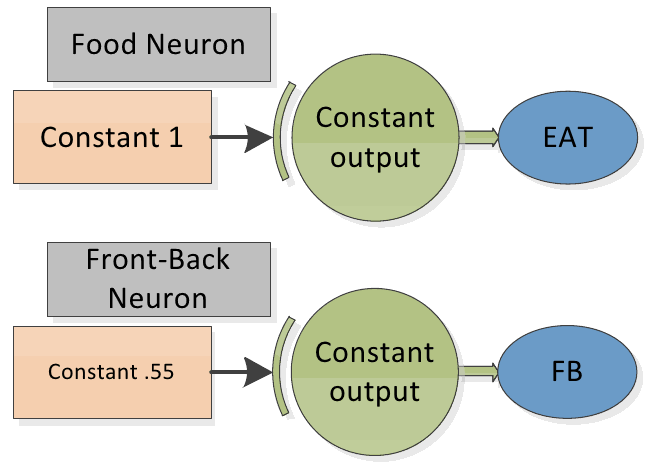
\includegraphics[scale=.3]{img/brain1.png}
  \caption{Active neurons in Brain 1}
  \label{fig:brain1}
\end{center}
\end{figure}

\subsection{Brain 2}

Brain 2 was the first neural network to take advantage of the agent's visual
cortex (fig. \ref{fig:brain2}). Of the 31 eyelets available to the agent, it 
used only the data it received from its center eyelet (eyelet 15). This
neuron instructs the agent to only use its eat actuator when it perceives
intense brightness. 

We caused this behavior by using a single neuron with a step function. 
The neuron was trained by having the agent try to eat at a variety of 
distances and observing the change in its charge. If the charge does not
change, then the brightness threshold is increased.

\begin{figure}
\begin{center}
  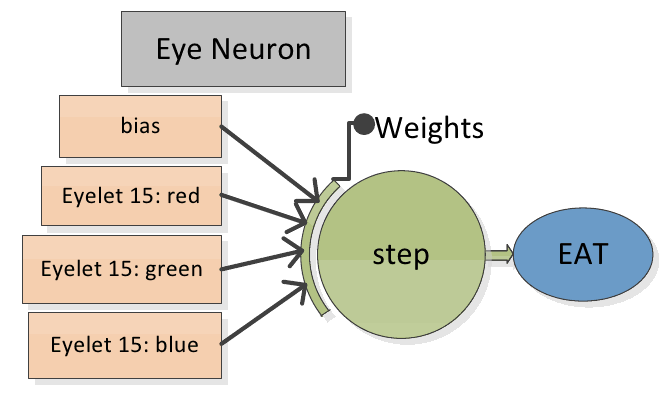
\includegraphics[scale=.3]{img/brain2.png}
  \caption{Brain 2's visual neuron}
  \label{fig:brain2}
\end{center}
\end{figure}

\subsection{Brain 3}

For Brain 3, we actually made two changes. The first was to the
eye neuron, which we changed from a step function to a sigmoid 
(fig. \ref{fig:brain3eye}):

\begin{equation} \label{eq:eyesig}
  \varphi(v) = \frac{\tanh(2v)}{10}
\end{equation}

We made this change because we wanted this model to focus on color. Whereas
our old step function classified \emph{all} objects as ``close enough'' vs. 
``not close enough,'' this new version could classify the color of an object by 
consuming it and comparing the output to the change in energy. Since this 
change 
can only be -0.1, 0, or 0.1, we selected a sigmoid function that would return 
a value within that range. Using a continuous function like equation 
\eqref{eq:eyesig} allows us to compare colors of objects.

\begin{figure}
\begin{center}
  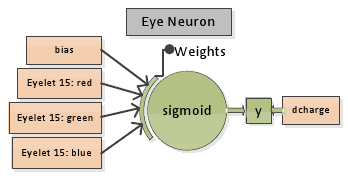
\includegraphics[scale=.7]{img/brain3eye.png}
  \caption{Brain 3's visual neuron}
  \label{fig:brain3eye}
\end{center}
\end{figure}

Our second change was to employ the somatic sensors of the agent
(fig. \ref{fig:brain3touch}). If the agent senses contact on any of its edges, 
it will eat. By using these somatic sensors, we keep our agent from slovenly
gnashing its teeth at every time step.

\begin{figure}
\begin{center}
  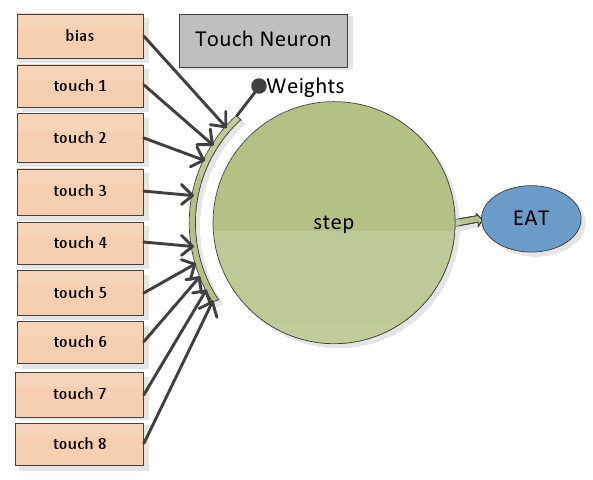
\includegraphics[scale=.5]{img/brain3touch2.png}
  \caption{Brain 3's somatic neuron}
  \label{fig:brain3touch}
\end{center}
\end{figure}

\subsection{Brain 4}

Our mission for Brain 4 was to implement the eyelets into a
winner-take-all network (fig. \ref{fig:brain4}). Each eyelet input is fed 
into two neurons: one \textbf{step function} to determine green/not green, and 
another 
which produced the linear summation of each color's intensity. These outputs
were fed into product neurons, which subsequently output to a 31-element WTA 
network. All 
neurons in this network connect to a single neuron that controls the rotation 
of the agent, and this neuron has fixed weights coming into it. Each of these 
weights correspond to an angle, which is the direction that eyelet is looking. 
These angles are used to instruct the agent where to turn.

\begin{figure}
\begin{center}
  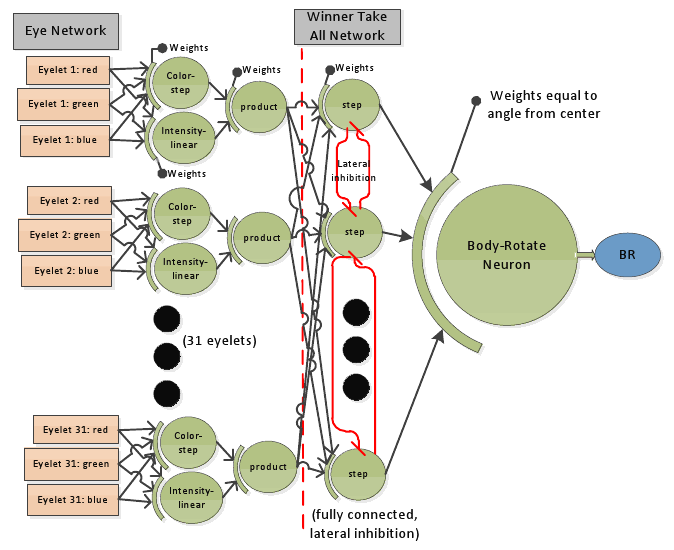
\includegraphics[scale=.52]{img/brain4.png}
  \caption{Brain 4's WTA eyelet network}
  \label{fig:brain4}
\end{center}
\end{figure}

\subsubsection{Waaaait a minute....}
We know what you're thinking. ``Step functions to determine color? But Brain 
3 introduced a sigmoid-based neuron!'' Indeed it is true. Furthermore, Brain
4 exerts no control over the eating actuator either. The reason for this is
that we, as the developers, simultaneously worked on Brains 3 and 4 separately.
Our initial thought was to fuse the two models together and toss the originals 
out. As you will see shortly, we did combine the two. However we kept Brains 
3 and 4 as a demonstration of a sort of evolutionary split in our agent's 
development. So without further ado...

\subsection{Brain 5}
Brain 5 applies the finer-grained sigmoid color neurons from 
fig. \ref{fig:brain3eye} to the augmented WTA network in 
fig. \ref{fig:brain4}. The object consumption is again determined by the 
somatic sensors from fig. \ref{fig:brain3touch}.

\subsection{Brain 6}
At this point in development, we wanted to refine the touch-and-munch nature
of our agent; why would it eat poison when it should know better? In order
to circumvent this greedy, potentially deadly tendency, we added a
color-based neuron to the agent's somatic-gastronomic system 
(fig. \ref{fig:brain6}). The somatic neuron will only fire if there is a
non-zero value for the ``mouth'' of the agent. Correspondingly, the
color-based neuron will only fire if an object in contact with it is green.
This is legal to assume, as the agent itself is aware of its own body. It will
never try to eat unless it has made contact with and object, and even then
will only do so if the object is green. This behavior is guaranteed by an
AND neuron, which serves as a gate between the touch and color neurons.

\begin{figure}
\begin{center}
  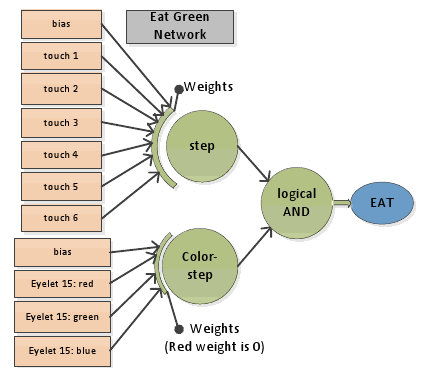
\includegraphics[scale=.7]{img/brain6.png}
  \caption{Brain 6's neural network for eating objects}
  \label{fig:brain6}
\end{center}
\end{figure}

\subsection{Brain 7}
\begin{figure}
\begin{center}
  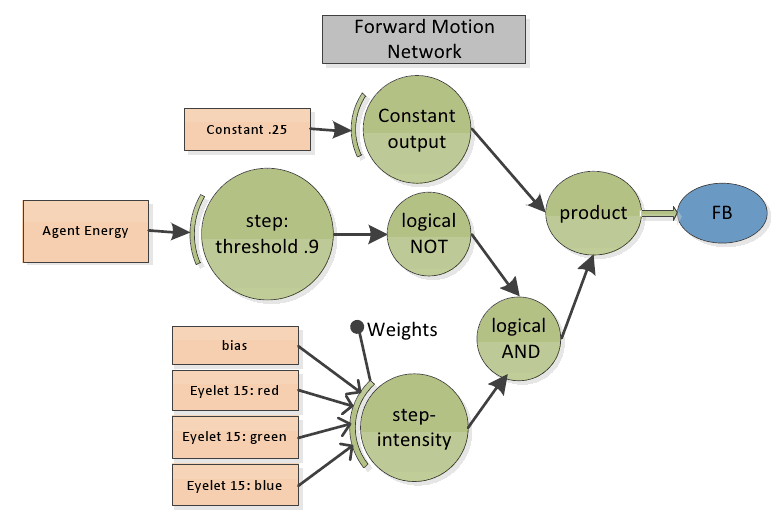
\includegraphics[scale=.5]{img/brain7.png}
  \caption{Brain 7's movement network near food}
  \label{fig:brain7}
\end{center}
\end{figure}

Our seventh and final brain addresses the issue of rationing food supplies in
Flatworld. As previously stated, our agent has a charge/lifespan that is defined
as a real number between 1 and 0, with 1 being a full charge and 0 meaning 
death. Food will increase the agent's charge by \emph{at most} +0.1. Eating 
a food object with a charge of 0.97 brings the agent's charge up to 1, a net
gain of +0.03. In order to get the most out of food objects, our agent
should never eat when it's not hungry. Fig. \ref{fig:brain7} describes our
network to help accomplish this goal.

 Most of the time the agent has the standard propulsion methods as it did in 
other models, fig. \ref{fig:brain7} is put into use under the special 
circumstances that our agent is very close to a food object, but is not hungry.
A constant value describes the forward movement rate (0.25 in this case). At 
every timestep the agent queries its internal charge. While its charge is 
$> 0.9$, the logical NOT will suppress the AND neuron, giving the 
forward/backward 
actuator a value of $0.25 \times 0 = 0$. Provided the object in question is 
close enough (described by the intensity neuron), when the agent's energy dips
below 0.9 the NOT neuron fires, the AND neuron is satisfied, and it fires a
non-zero value to the product neuron.

\section{Results} \label{sec:Results}

%%%%%%%%%%%%%%%%%%%%%%%%%%%%%%%%%%%%%%%%%%%%%%%%%%%%%%%%%%%%%%%%%%%%%%%%%%%  
%% JUST THE OBJECTIVE FACTS, no interpretation or discussion
%%
%% what exactly did you do
%%  
%% what were the inputs/outputs/parameters
%%  
%% what computer hardware
%%  
%% what software
%%  
%% what were the results
%%  
%% tables/figures/plots
%%  
%% error analysis
%%%%%%%%%%%%%%%%%%%%%%%%%%%%%%%%%%%%%%%%%%%%%%%%%%%%%%%%%%%%%%%%%%%%%%%%%%%  

Here we shall present the results we acquired from our experiments. We will
describe our generic testbed, so should the reader wish to follow along in
real time they may have the option of doing so. After this, the performance 
of each brain will be evaluated individually.

\subsection{Testbed}
All of our experiments were performed within the Flatworld II v.1.0 
environment. Our code was writen in Python 2.6, and interfaced with 
Flatworld's C-based API via a shim (see section \ref{sec:Ack}). All of our
runs were done on a Lenovo Ideapad T430 with an Intel i7 quad core processor
and 16GB of DDR3 RAM. Windows 7 Pro 64bit is the machine's native platform,
but we ran our tests inside a virtual machine using VMware 8.04. The virtual
machine was configured with Ubuntu 10.04 32bit, 1GB of RAM and a single 2GHz
processor. We used Matplotlib 1.2 for our data figures.


\subsection{Brain 0}
We start our data presentation with Brain 0 (a very good place to start).
It should come as no surprise that brain 0's lifespan is 2000 time steps. 
The agent makes no moves, and makes no attempts to eat anything. 
Figure \ref{fig:brain0energy} shows an agent's average energy depletion over 
time based upon 153 runs. The bar has been set, as they say.

\begin{figure}
\begin{center}
  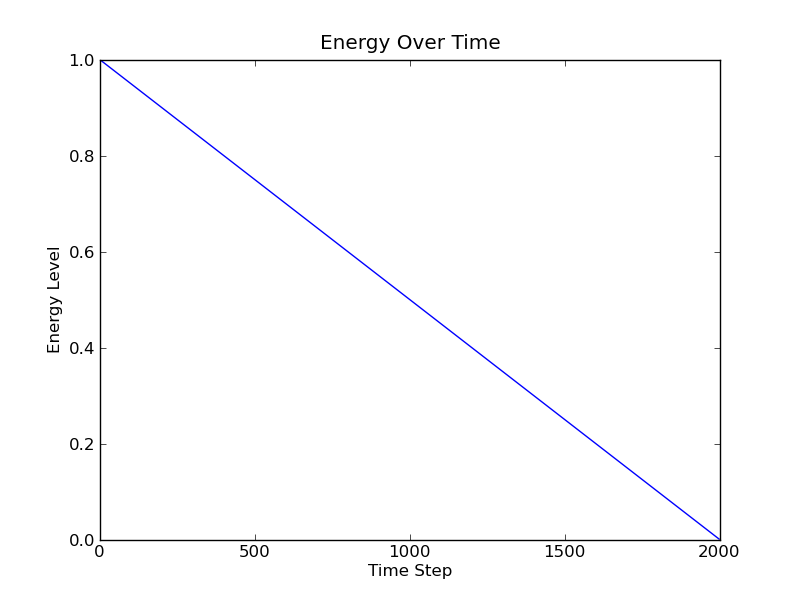
\includegraphics[scale=.65]{plots/brain0energy.png}
  \caption{Agent's energy level over time ($\sigma = 0$)}
  \label{fig:brain0energy}
\end{center}
\end{figure}

Figure \ref{fig:brain0his} is a histogram which also confirms the average 
lifespan of our agents to be exactly 2000 time steps.

\begin{figure}
\begin{center}
  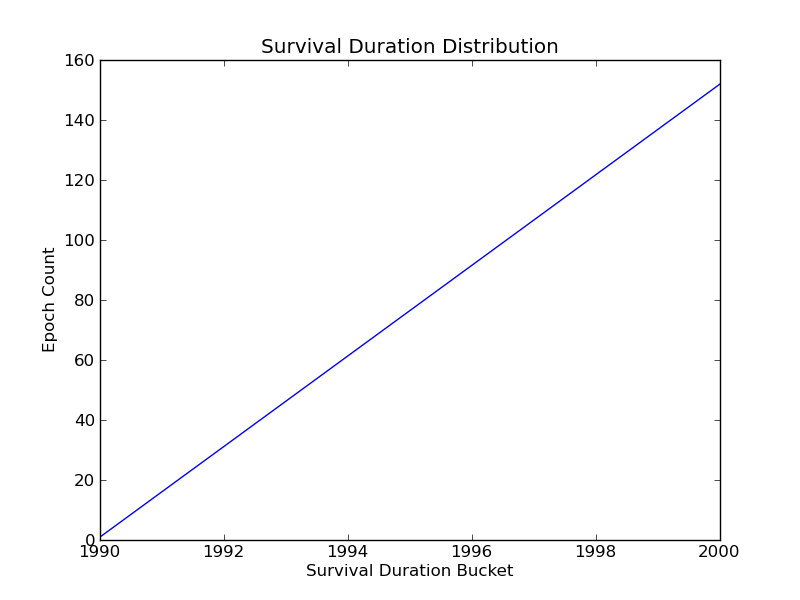
\includegraphics[scale=.65]{plots/brain0hist.png}
  \caption{Agent lifetimes for Brain 0 ($\sigma = 0$)\\
  (Note: this is Matplotlib's attempt to plot a linear distribution of
  a single data point)}
  \label{fig:brain0his}
\end{center}
\end{figure}


\subsection{Brain 1}
It should come as no surprise that Brain 1's performance will show
little improvement upon Brain 0. This is due to the fact that not only is
it relying on food to be directly in its path, but it also is expending 
\emph{more} energy from the act of moving. Figure \ref{fig:brain1velo} shows
that increasing the agent's velocity will cause its energy to decrease
exponentially.

\begin{figure}
\begin{center}
  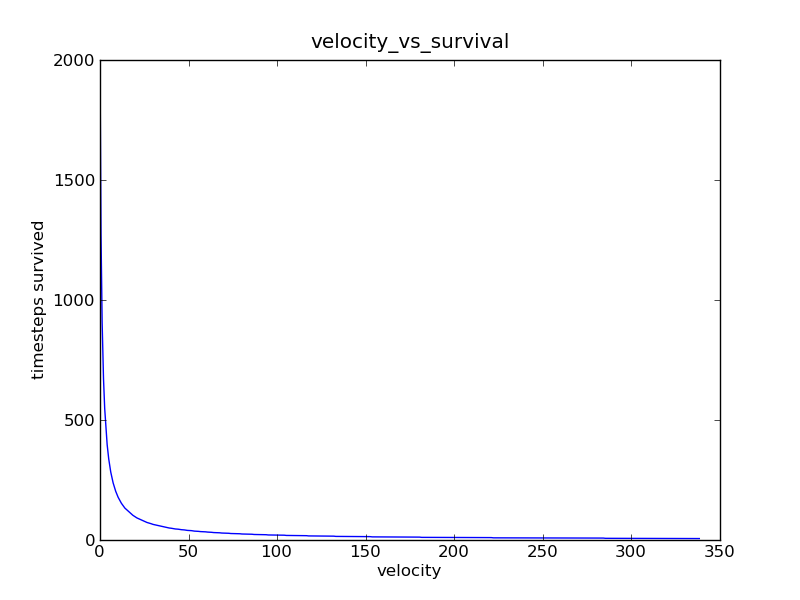
\includegraphics[scale=.65]{plots/brain1velo.png}
  \caption{An agent's lifespan as a function of velocity}
  \label{fig:brain1velo}
\end{center}
\end{figure}

\begin{figure}
\begin{center}
  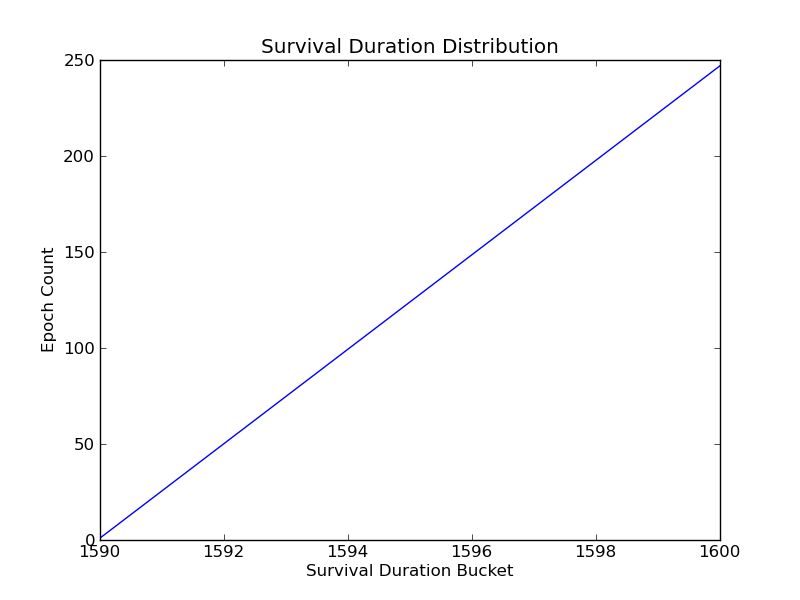
\includegraphics[scale=.65]{plots/brain1hist.png}
  \caption{Agent lifetimes for Brain 1 ($\sigma = 0.11$)\\
  (Again... Matplotlib)}
  \label{fig:brain1his}
\end{center}
\end{figure}

The histogram in figure \ref{fig:brain1his} illustrates agents' lifetimes based
off of a constant velocity value of 0.25. There was very, very little change
in lifetime from run to run. The average survival time of 248 runs was 
1600.00.

\subsection{Brain 2}
Brain 2 performed less effectively than Brain 1, despite the addition of the
eyelet neuron. The average lifespan for agents endowed with Brain 2 was 
1557.85.

\begin{figure}
\begin{center}
  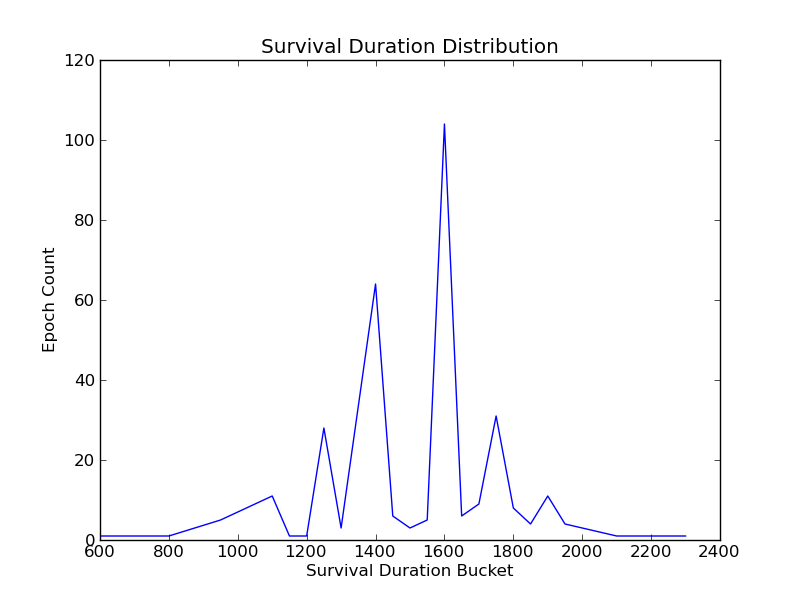
\includegraphics[scale=.65]{plots/brain2hist.png}
  \caption{Agent lifetimes for Brain 2 ($\sigma = 227.88$)}
  \label{fig:brain2his}
\end{center}
\end{figure}

\subsection{Brain 3}

\begin{figure}
\begin{center}
  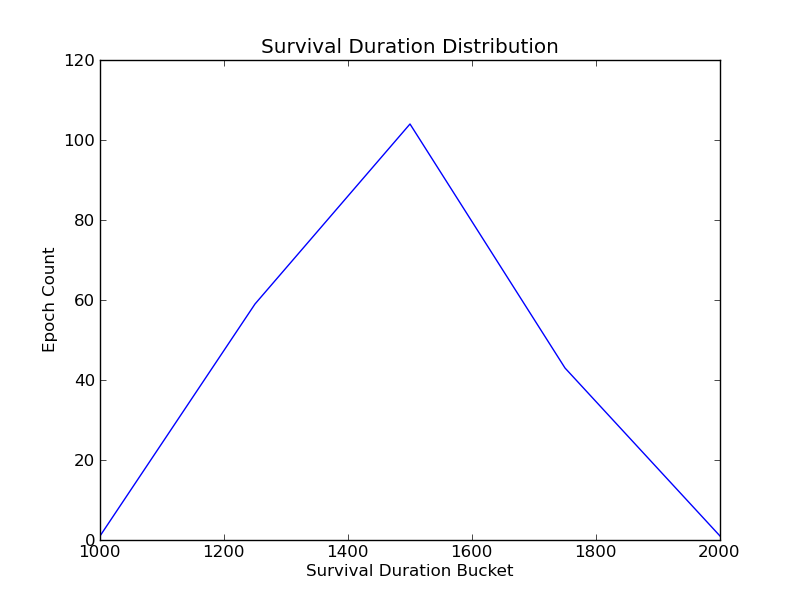
\includegraphics[scale=.65]{plots/brain3hist.png}
  \caption{Agent lifetimes for Brain 3 ($\sigma = 153.55$)}
  \label{fig:brain3his}
\end{center}
\end{figure}

Brain 3, which introduced the sigmoid neuron, also performed more poorly
than Brain 0, with a an average lifespan of 1581.63. The standard deviation
improved from Brain 2, though.

\begin{figure}
\begin{center}
  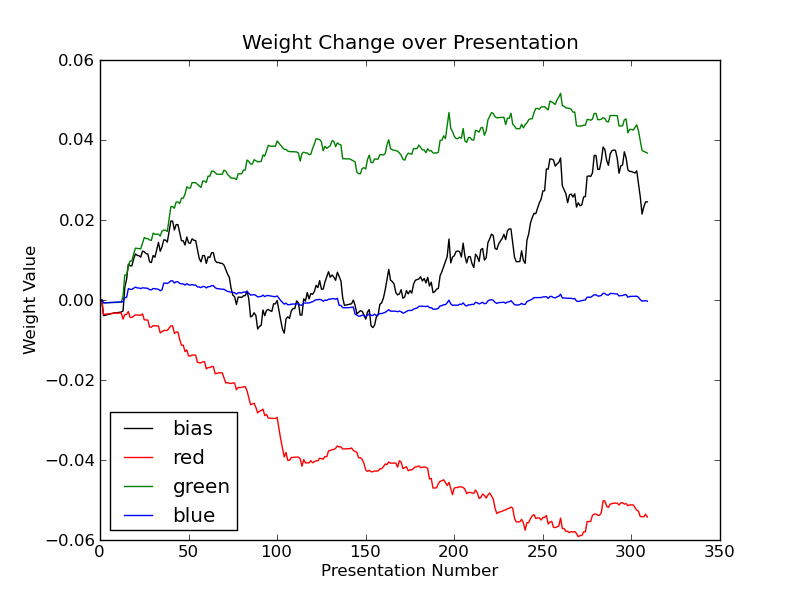
\includegraphics[scale=.65]{plots/weights.png}
  \caption{Weight change for sigmoid neuron}
  \label{fig:brain3wghts}
\end{center}
\end{figure}

Also, via figure \ref{fig:brain3wghts}, you can see that the sigmoid neuron 
was behaving properly; weights were
adjusted after viewing each object using the formula\cite{Haykin}

\begin{equation}
  w_i(n+1) = w_i + \eta e(n) \varphi'(n) x_i(n)
\end{equation}

What we were left with is a high food probability with a positive output,
a high poison probability with negative outputs, and a likely neutral object 
for very, very small outputs.

At this point we should mention that, after we had gotten satisfactory 
convergence, we decided to turn off learning for the sigmoid neuron(s) and use 
hard-coded values. The trial runs we had for Brain 3 proved that our color
classifier neuron was indeed doing its job.


\subsection{Brain 4}

\begin{figure}
\begin{center}
  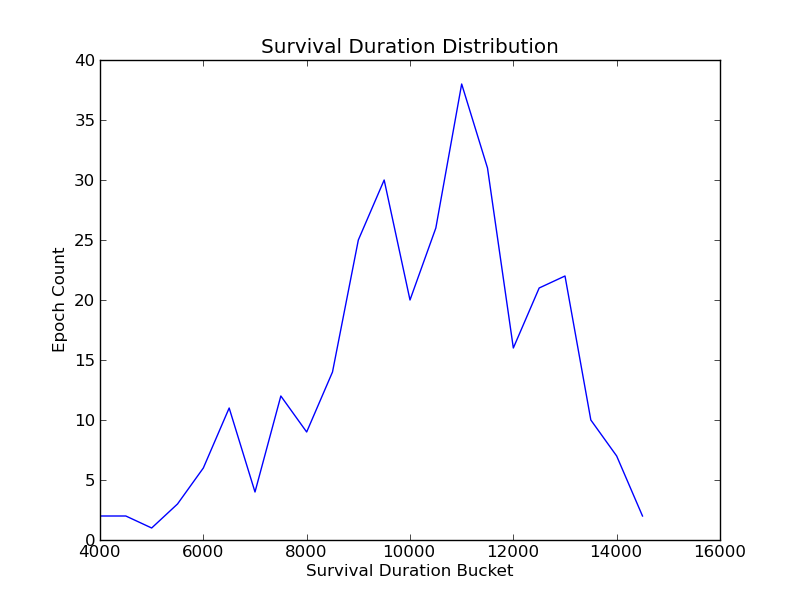
\includegraphics[scale=.65]{plots/brain4hist.png}
  \caption{Agent lifetimes for Brain 4 ($\sigma = 2154.90$)}
  \label{fig:brain4his}
\end{center}
\end{figure}

Agents sporting Brain 4 lived to ripe ages that has not been seen in previous
models (fig. \ref{fig:brain4his}); sporting an average lifespan of 12480. This is also 
the first Brain 
to implement a WTA network for the visual cortex and allow for directional 
change.


\subsection{Brain 5}

\begin{figure}
\begin{center}
  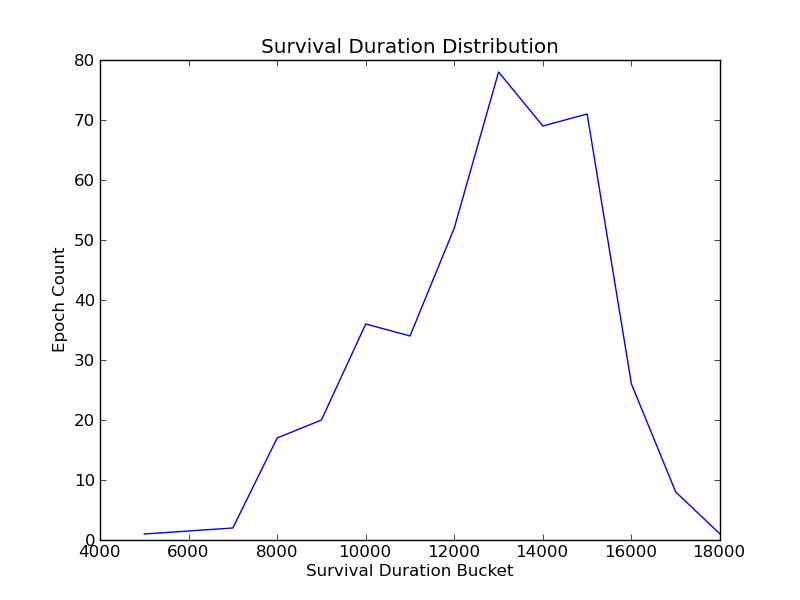
\includegraphics[scale=.65]{plots/brain5hist.png}
  \caption{Agent lifetimes for Brain 5 ($\sigma = 2289.75$)}
  \label{fig:brain5his}
\end{center}
\end{figure}

Brain 5 is the combination of Brains 3 and 4. The average lifetime for 446
agents with Brain 5 was 13238; despite the combination, that netted just 
slightly less than a 6\% improvement over Brain 4's average lifetime. 


\subsection{Brain 6}
\begin{figure}
\begin{center}
  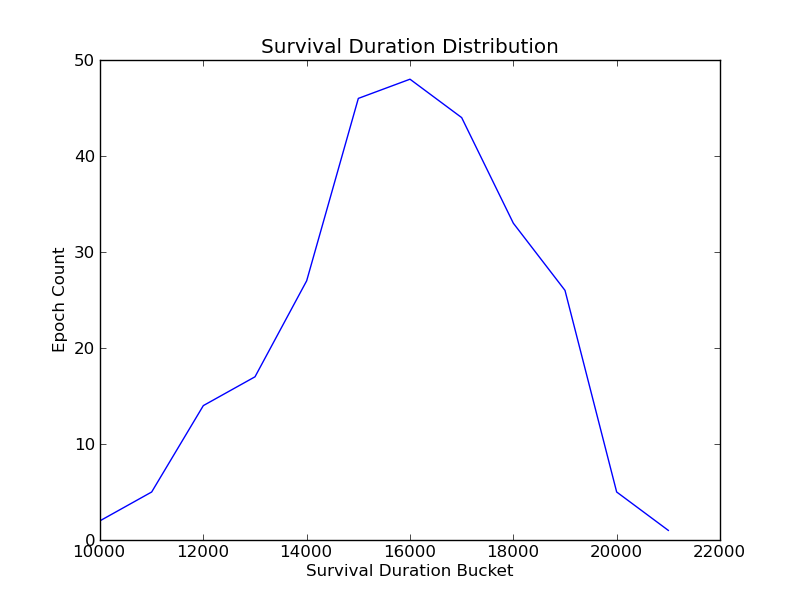
\includegraphics[scale=.65]{plots/brain6hist.png}
  \caption{Agent lifetimes for Brain 6 ($\sigma = 2143.33$)}
  \label{fig:brain6his}
\end{center}
\end{figure}

Agents equipped with Brain 6, who consider object color before causing the 
agent to eat, saw further improvement (fig. \ref{fig:brain6his}). The average 
time-to-death of the agents was 16374.08. The standard deviation also decreased.


\subsection{Brain 7}
\begin{figure}
\begin{center}
  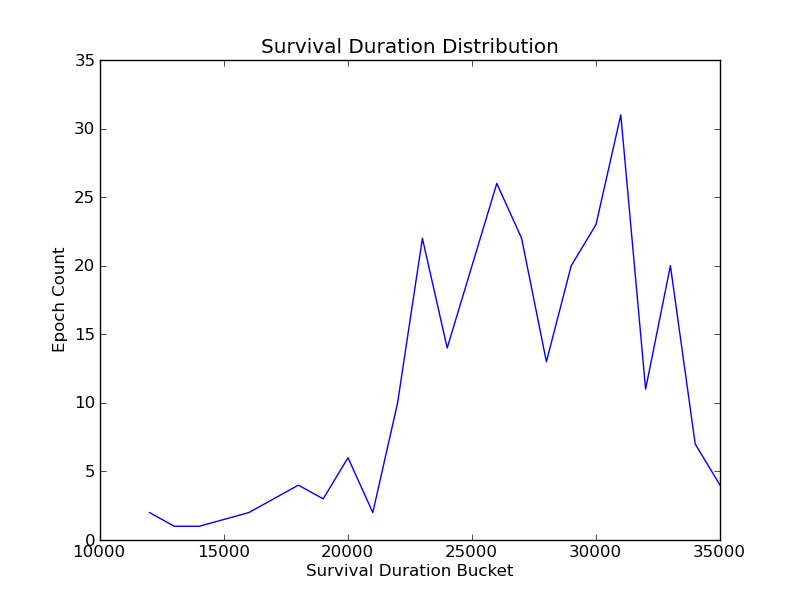
\includegraphics[scale=.65]{plots/brain7hist.png}
  \caption{Agent lifetimes for Brain 7 ($\sigma = 4523.73$)}
  \label{fig:brain7his}
\end{center}
\end{figure}

Brain 7 saw another massive jump in the agents' vitality 
(fig. \ref{fig:brain7his}). An average lifetime of 27623.54 is an improvement
of approximately 40\% over Brain 6. Note, too, that there is a large increase 
in the standard deviation of those lifetimes.


\subsection{Brain Comparison}
\begin{figure}
\begin{center}
  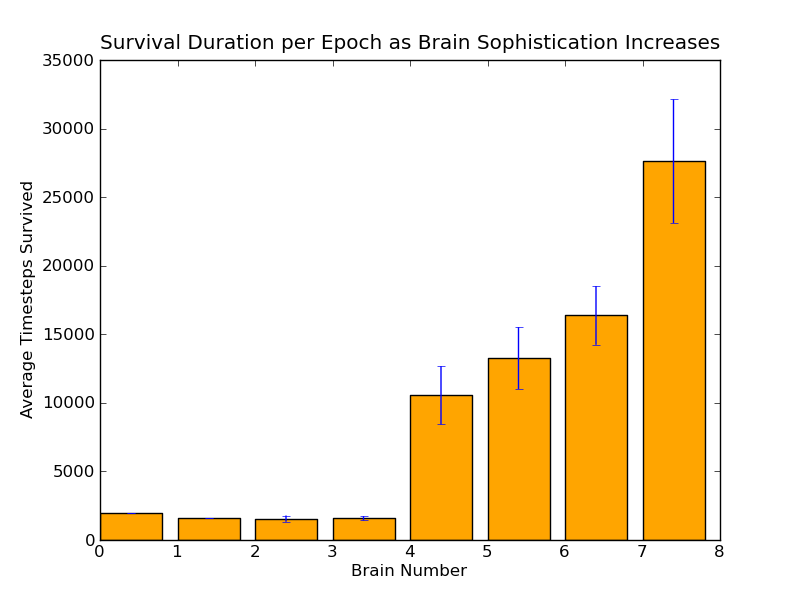
\includegraphics[scale=.65]{plots/survive.png}
  \caption{Agent lifetimes across all 8 brains}
  \label{fig:survive}
\end{center}
\end{figure}

Figure \ref{fig:survive} shows a side-by-side comparison of an agent's 
projected lifespan given its brain model.

\documentclass[a4paper,11pt]{article}
\begin{document}


\section{Discussion} \label{sec:Discussion}

\begin{itemize}
   \item
     your opinion of the study.
   \item
     your opinion of the results
   \item
     interpretations
   \item
     comments
   \item
     analysis
   \item
     what was right/wrong
   \item
     improvements
   \item
     connections back to the literature
\end{itemize}
\end{document}
\section{Summary} \label{sec:Summary}
\begin{itemize}
  \item
    the topic
  \item
    the problem
  \item
    other's solutions
  \item        
    your solution
  \item
    what was right/wrong about it
  \item
    future work
  \item
    conclusion 
\end{itemize}

\section{Acknowledgements} \label{sec:Ack}
\begin{itemize}
  \item
    someone must have helped in some way (Nasser for one)
  \item
    funding agencies, centers, departments
\end{itemize}

\appendix

%Import our appendices here:


\documentclass[a4paper,11pt]{article}
\usepackage{graphicx}


\begin{document}

\section{Model Architecture} \label{ap:arch}

\begin{figure}
\begin{center}
  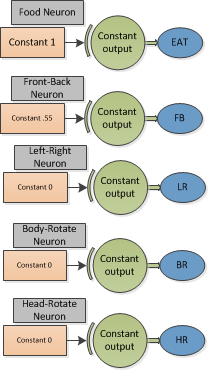
\includegraphics[scale=1.0]{img/brain1complete.png}
  \caption{Complete Neural Architecture for Brain1 }
  \label{fig:brain1complete}
\end{center}
\end{figure}

\begin{figure}
\begin{center}
  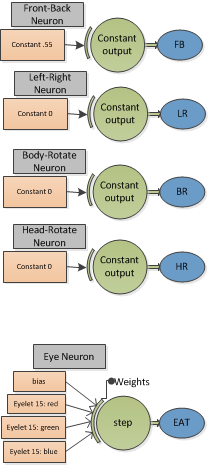
\includegraphics[scale=1.0]{img/brain2complete.png}
  \caption{Complete Neural Architecture for Brain2 }
  \label{fig:brain2complete}
\end{center}
\end{figure}


\begin{figure}
\begin{center}
  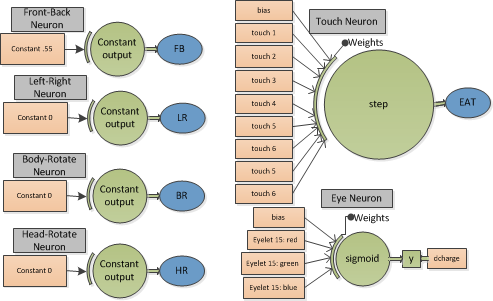
\includegraphics[scale=1.0]{img/brain3complete.png}
  \caption{Complete Neural Architecture for Brain3 }
  \label{fig:brain3complete}
\end{center}
\end{figure}


\begin{figure}
\begin{center}
  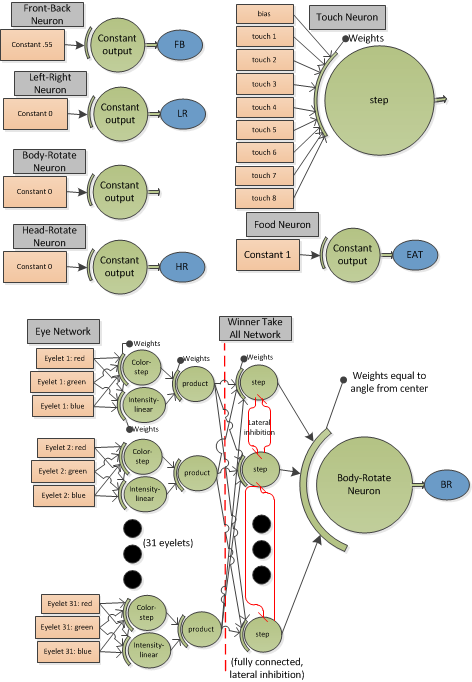
\includegraphics[scale=1.0]{img/brain4complete.png}
  \caption{Complete Neural Architecture for Brain4 }
  \label{fig:brain4complete}
\end{center}
\end{figure}


\begin{figure}
\begin{center}
  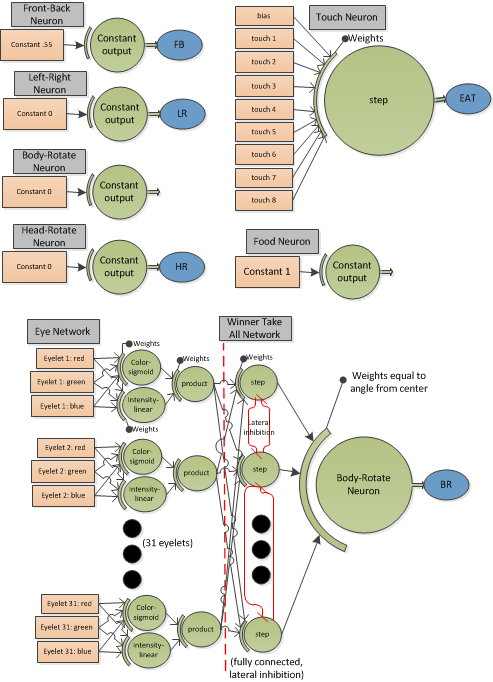
\includegraphics[scale=1.0]{img/brain5complete.png}
  \caption{Complete Neural Architecture for Brain5 }
  \label{fig:brain5complete}
\end{center}
\end{figure}


\begin{figure}
\begin{center}
  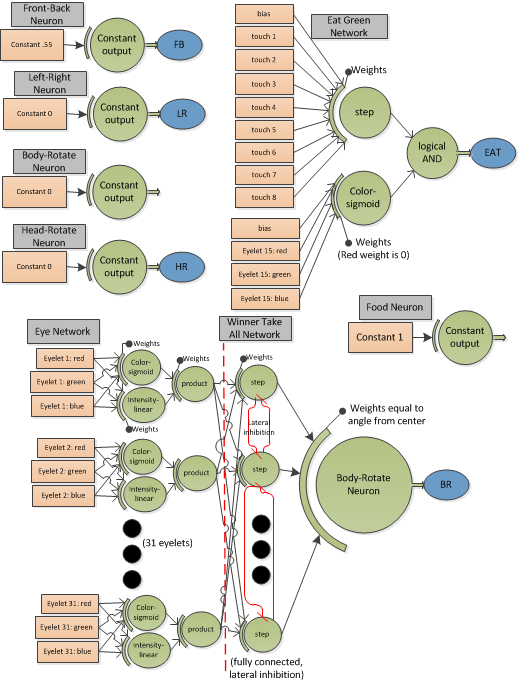
\includegraphics[scale=1.0]{img/brain6complete.png}
  \caption{Complete Neural Architecture for Brain6 }
  \label{fig:brain6complete}
\end{center}
\end{figure}


\begin{figure}
\begin{center}
  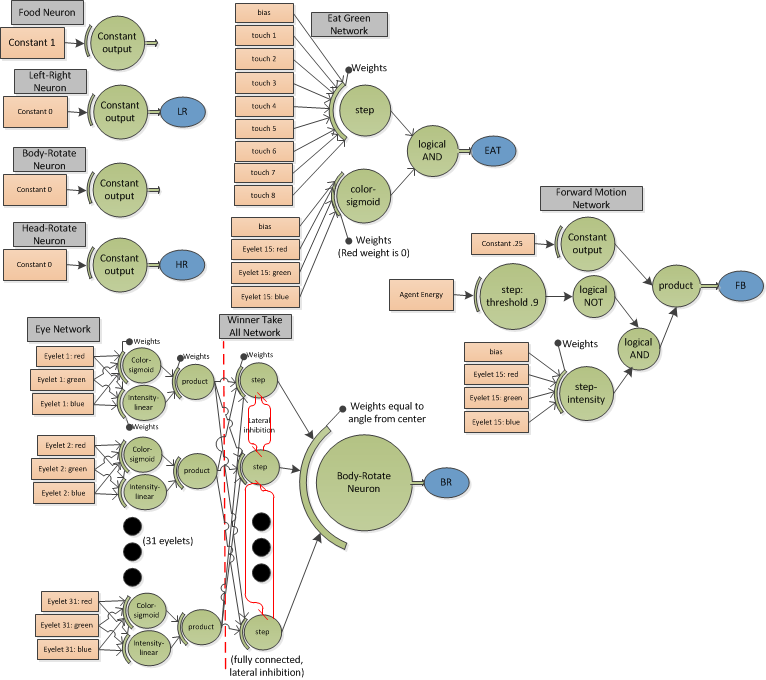
\includegraphics[scale=1.0]{img/brain7complete.png}
  \caption{Complete Neural Architecture for Brain7 }
  \label{fig:brain7complete}
\end{center}
\end{figure}

\begin{figure}
\begin{center}
  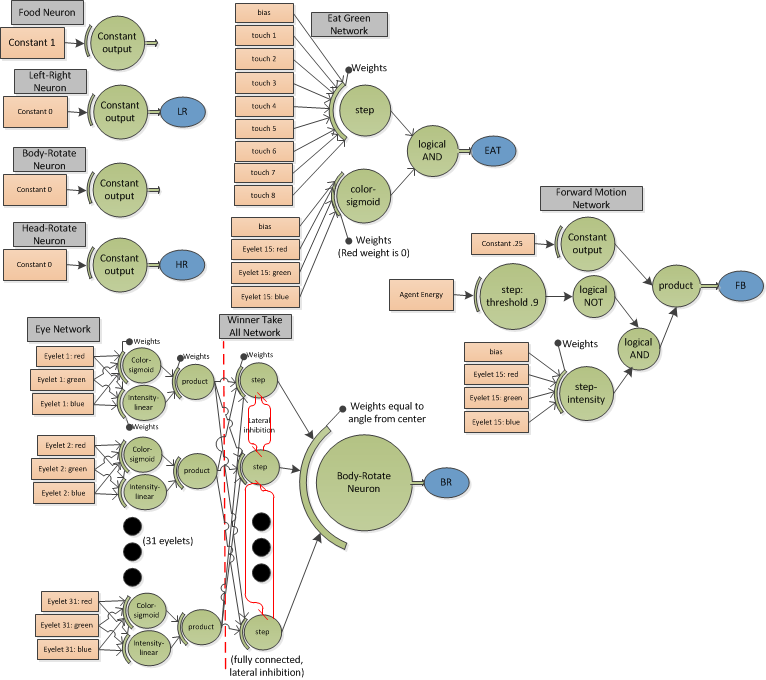
\includegraphics[scale=1.0]{img/brain7complete.png}
  \caption{Complete Neural Architecture for Brain7 }
  \label{fig:brain7complete}
\end{center}
\end{figure}

\begin{figure}
\begin{center}
  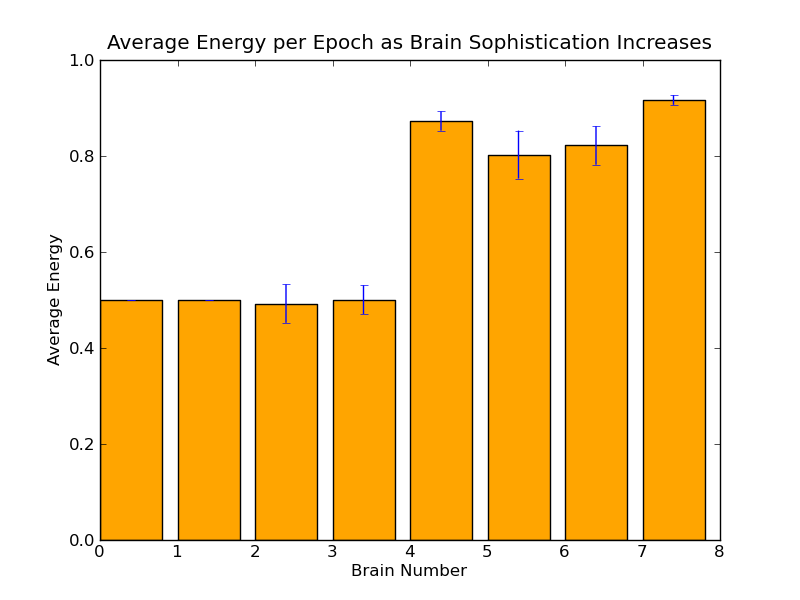
\includegraphics[scale=1.0]{img/avgEnergyBar-0.0-0.0-0.04-0.03-0.02-0.05-0.04-0.01.png}
  \caption{Average Average-Energy of Agent per Epoch per Brain }
  \label{fig:avgenergybar}
\end{center}
\end{figure}

\begin{figure}
\begin{center}
  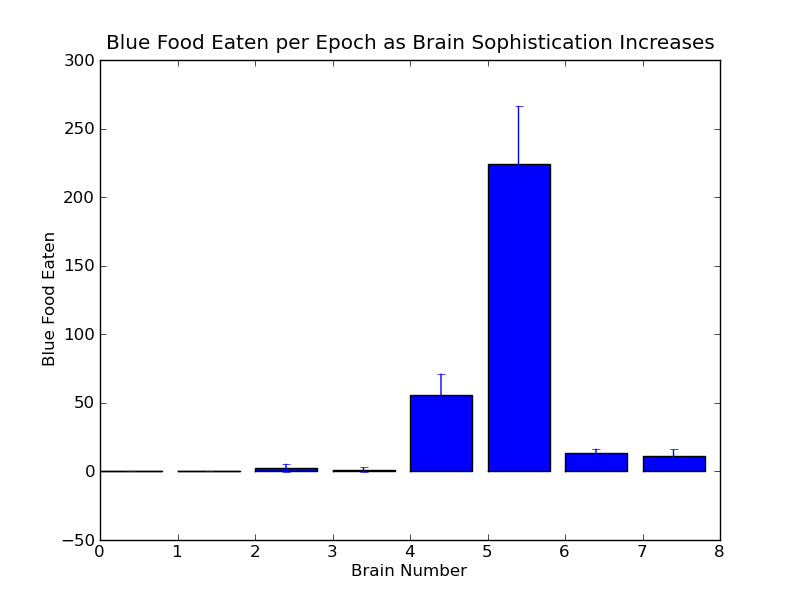
\includegraphics[scale=1.0]{img/blueBar-0.0-0.0-2.85-1.76-15.72-42.67-3.31-4.54.png}
  \caption{Average Neutral Food Items Consumed per Epoch per Brain }
  \label{fig:bluebar}
\end{center}
\end{figure}

\begin{figure}
\begin{center}
  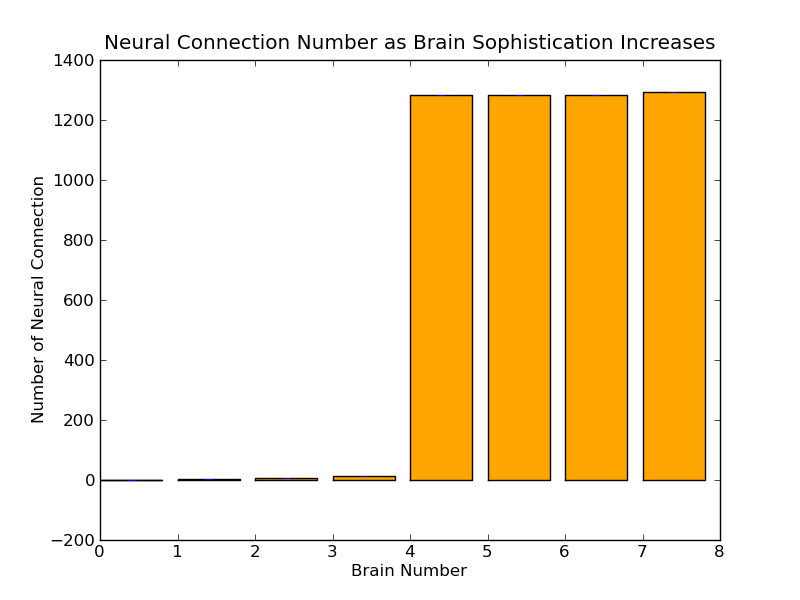
\includegraphics[scale=1.0]{img/connectionBar-0.0-0.0-0.0-0.0-0.0-0.0-0.0-0.0.png}
  \caption{Summation of Input Neurons over all Neurons }
  \label{fig:connectionbar}
\end{center}
\end{figure}

\begin{figure}
\begin{center}
  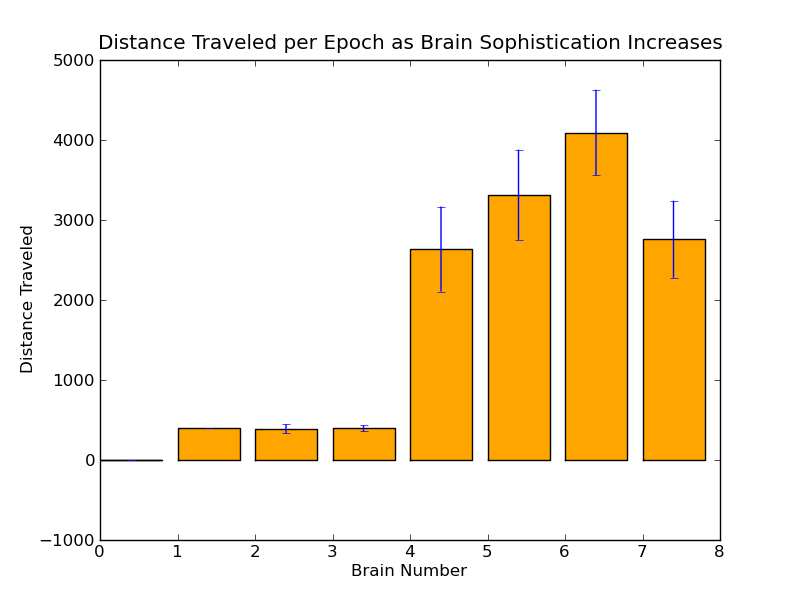
\includegraphics[scale=1.0]{img/distanceBar-0.0-0.0-56.89-38.55-531.39-563.6-534.63-481.99.png}
  \caption{Average Total Distance Traveled per Epoch per Brain }
  \label{fig:distancebar}
\end{center}
\end{figure}

\begin{figure}
\begin{center}
  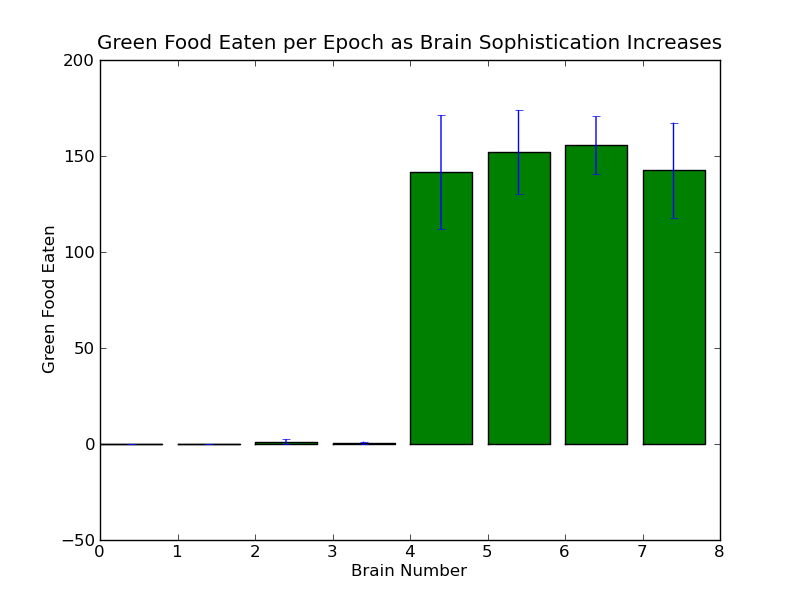
\includegraphics[scale=1.0]{img/greenBar-0.0-0.0-1.32-0.69-29.79-21.82-15.12-24.72.png}
  \caption{Average Healthy Food Items Consumed per Epoch per Brain  }
  \label{fig:greenbar}
\end{center}
\end{figure}

\begin{figure}
\begin{center}
  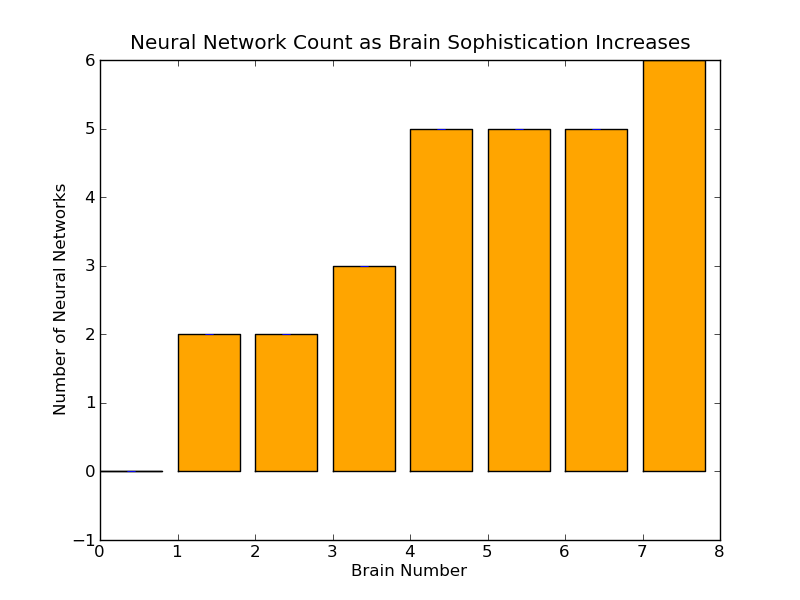
\includegraphics[scale=1.0]{img/networkBar-0.0-0.0-0.0-0.0-0.0-0.0-0.0-0.0.png}
  \caption{Number of Independent Neural Networks per Brain }
  \label{fig:networkbar}
\end{center}
\end{figure}

\begin{figure}
\begin{center}
  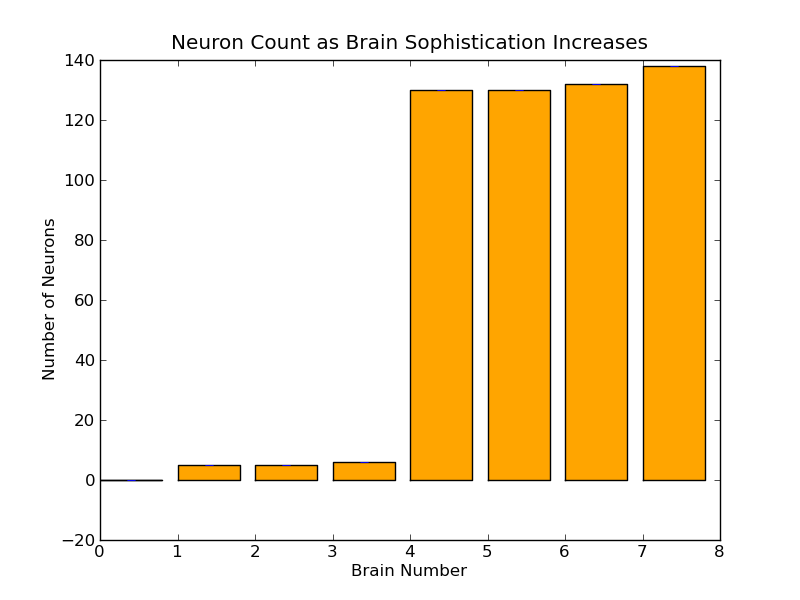
\includegraphics[scale=1.0]{img/neuronBar-0.0-0.0-0.0-0.0-0.0-0.0-0.0-0.0.png}
  \caption{Total Number of Neurons per Brain }
  \label{fig:neuronbar}
\end{center}
\end{figure}

\begin{figure}
\begin{center}
  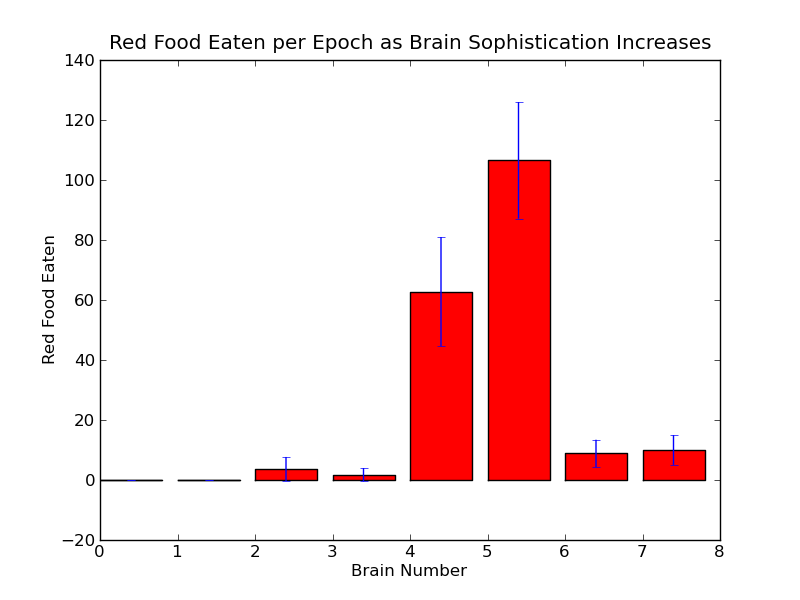
\includegraphics[scale=1.0]{img/redBar-0.0-0.0-4.0-2.23-18.21-19.44-4.58-4.97.png}
  \caption{Average Poison Food Items Consumed per Epoch per Brain  }
  \label{fig:redbar}
\end{center}
\end{figure}

\begin{figure}
\begin{center}
  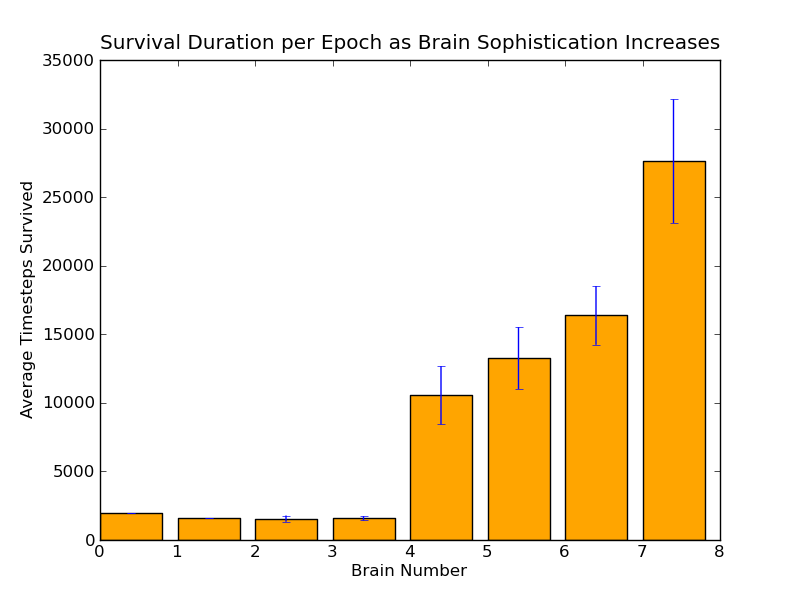
\includegraphics[scale=1.0]{img/survivalBar-0.11-0.11-227.69-154.23-2125.55-2254.41-2138.59-4506.76.png}
  \caption{Average Number of Time Steps Survived per Epoch per Brain}
  \label{fig:survivalbar}
\end{center}
\end{figure}













%brain 1
\begin{figure}
\begin{center}
  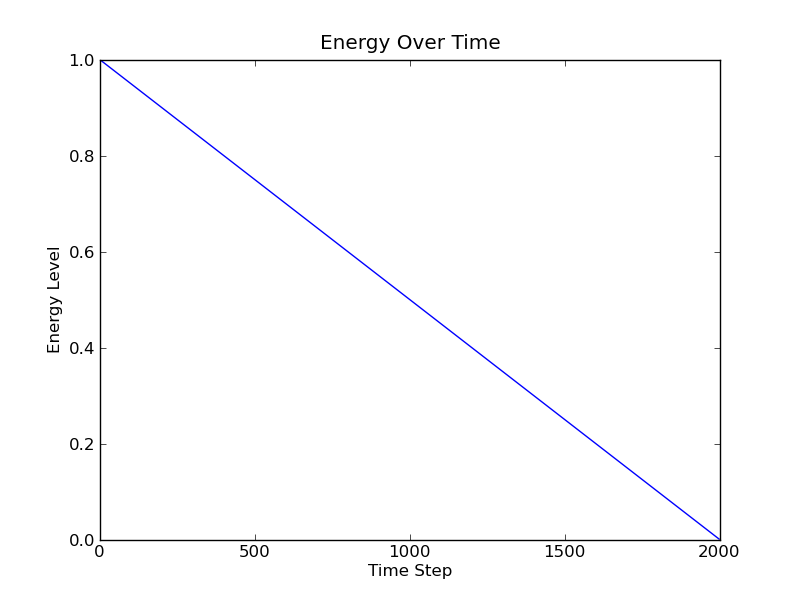
\includegraphics[scale=1.0]{img/brain1/1353130043-0.250000-EvT.png}
  \caption{Brain 1 Energy over Time for a Random Epoch}
  \label{fig:b1evt}
\end{center}
\end{figure}

\begin{figure}
\begin{center}
  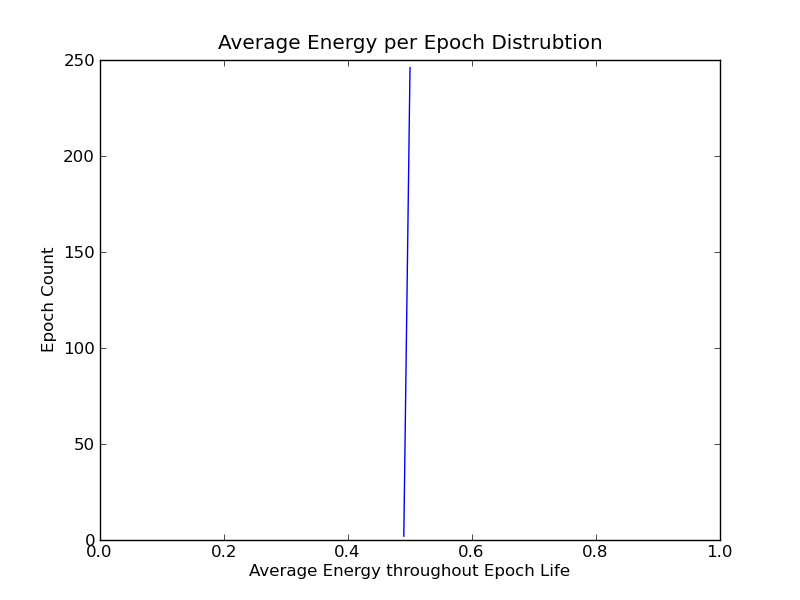
\includegraphics[scale=1.0]{img/brain1/avgenergyGauss-0.01.png}
  \caption{Brain 1 Distribution of Average Energies per Epoch}
  \label{fig:b1avgenergy}
\end{center}
\end{figure}








%brain 2
\begin{figure}
\begin{center}
  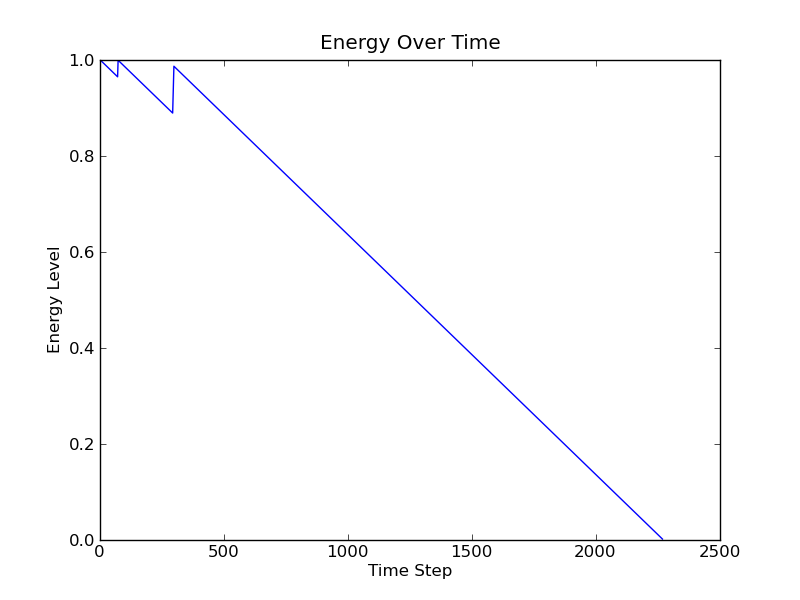
\includegraphics[scale=1.0]{img/brain2/1353128412-0.250000-EvT.png}
  \caption{Brain 2 Energy over Time for a Random Epoch}
  \label{fig:b2evt}
\end{center}
\end{figure}

\begin{figure}
\begin{center}
  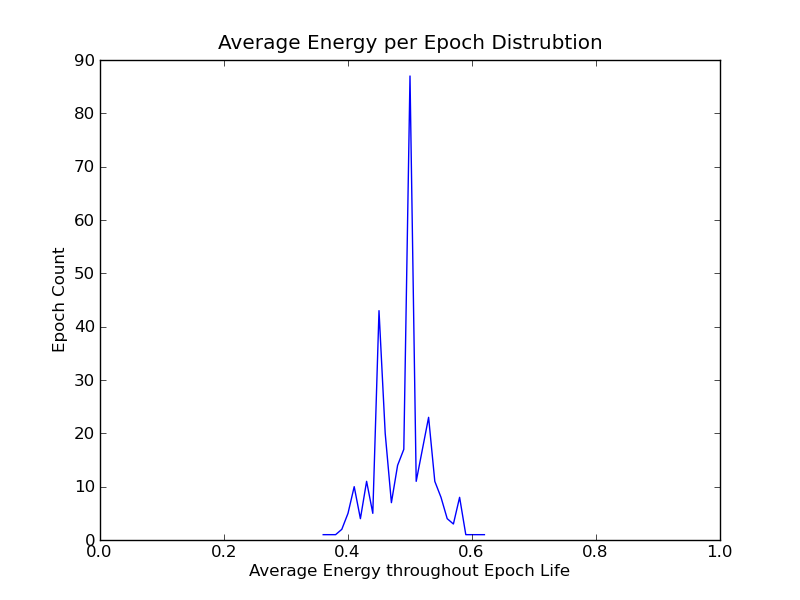
\includegraphics[scale=1.0]{img/brain2/avgenergyGauss-0.07.png}
  \caption{Brain 2 Distribution of Average Energies per Epoch}
  \label{fig:b2avgenergy}
\end{center}
\end{figure}

\begin{figure}
\begin{center}
  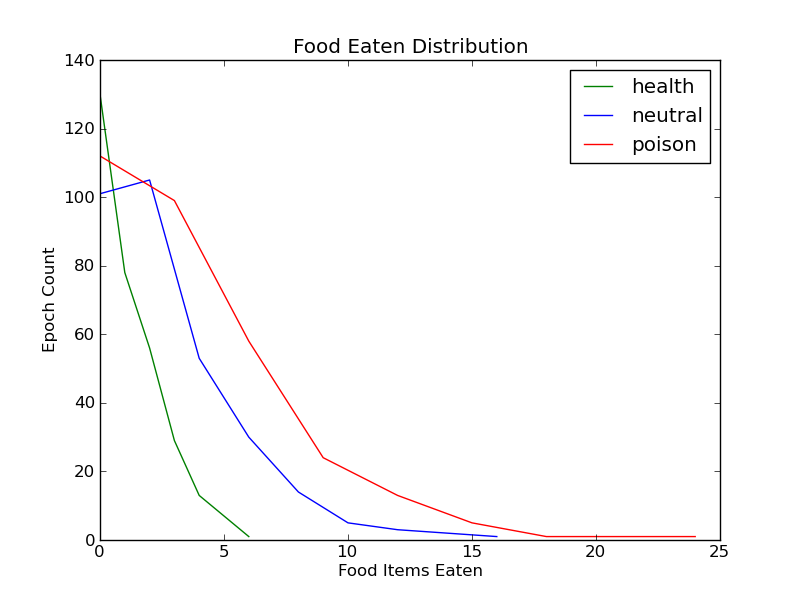
\includegraphics[scale=1.0]{img/brain2/foodGauss-h2.0-n5.16-p7.75.png}
  \caption{Brain 2 Distribution of Food Items Eaten per Epoch}
  \label{fig:b2food}
\end{center}
\end{figure}

\begin{figure}
\begin{center}
  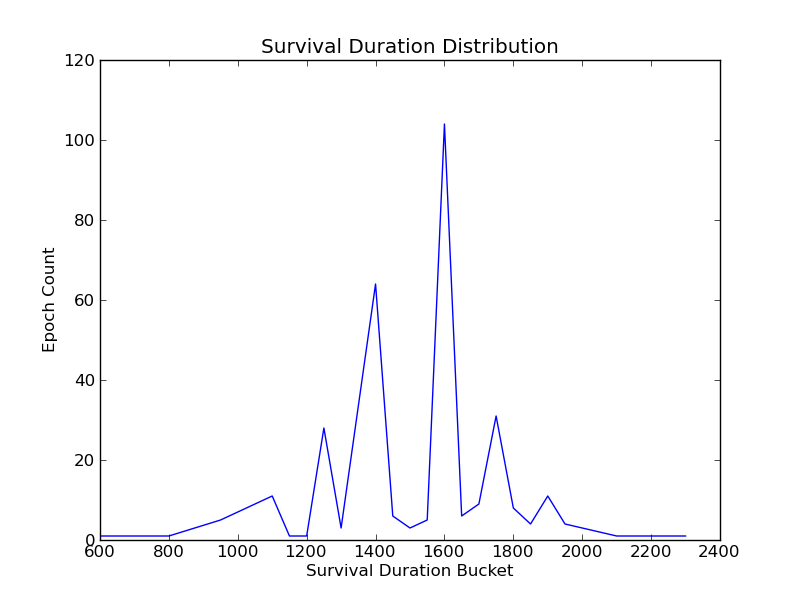
\includegraphics[scale=1.0]{img/brain2/survivalGauss-435.55.png}
  \caption{Brain 2 Distribution of Time Steps Survived per Epoch}
  \label{fig:b2survive}
\end{center}
\end{figure}

\begin{figure}
\begin{center}
  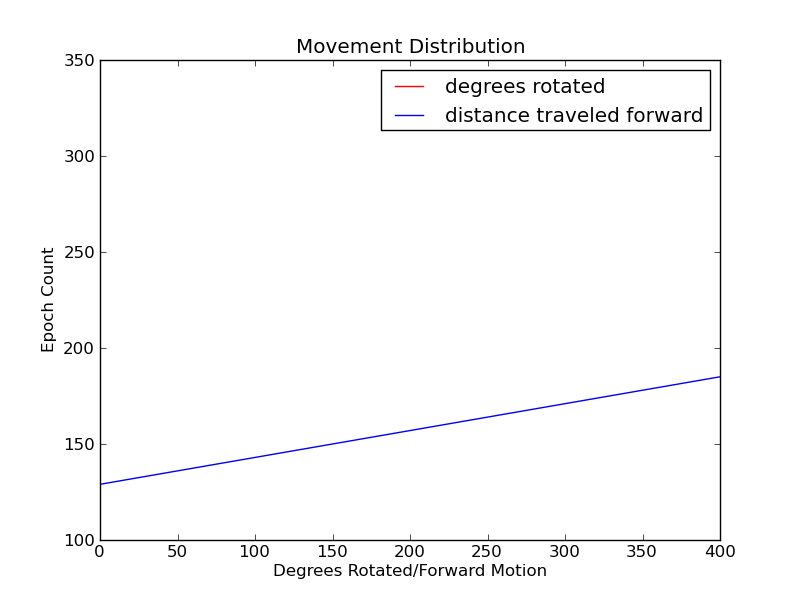
\includegraphics[scale=1.0]{img/brain2/travelGauss-r0.00-d200.00.png}
  \caption{Brain 2 Distribution of Number of Degrees Rotated and Units Travelled Forward per Epoch}
  \label{fig:b2travel}
\end{center}
\end{figure}









%brain 3

\begin{figure}
\begin{center}
  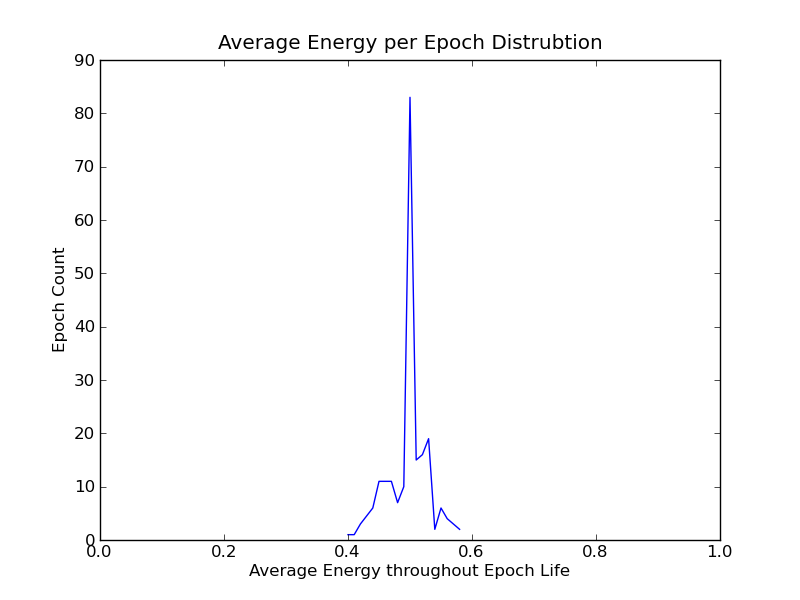
\includegraphics[scale=1.0]{img/brain3/avgenergyGauss-0.05.png}
  \caption{Brain 3 Distribution of Average Energies per Epoch}
  \label{fig:b3avgenergy}
\end{center}
\end{figure}

\begin{figure}
\begin{center}
  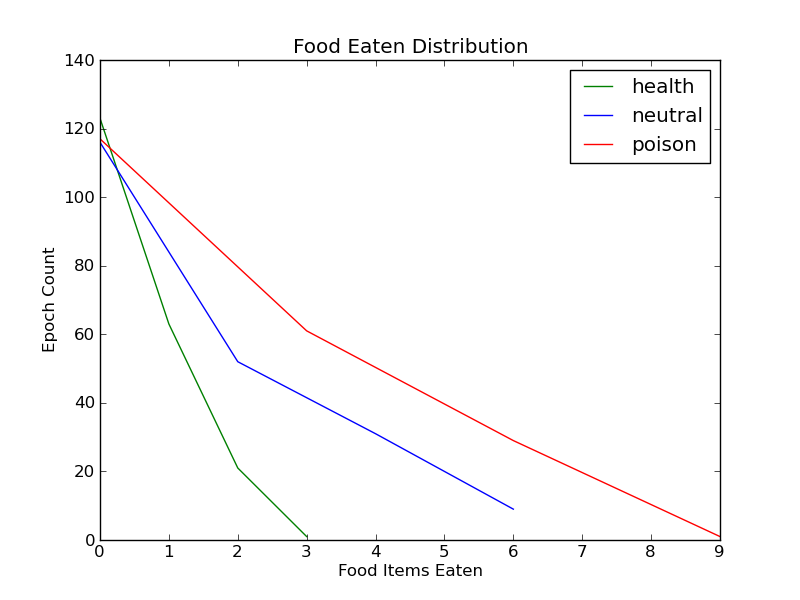
\includegraphics[scale=1.0]{img/brain3/foodGauss-h1.12-n2.24-p3.35.png}
  \caption{Brain 3 Distribution of Food Items Eaten per Epoch}
  \label{fig:b3food}
\end{center}
\end{figure}

\begin{figure}
\begin{center}
  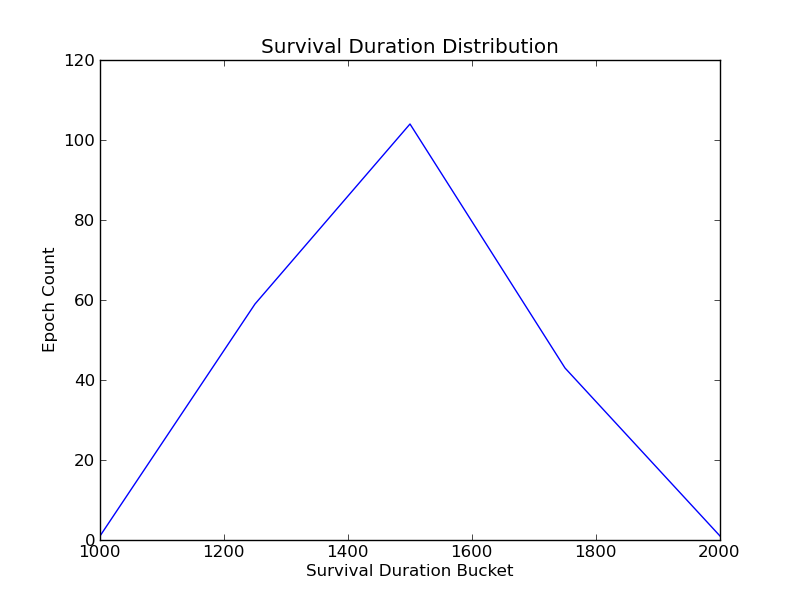
\includegraphics[scale=1.0]{img/brain3/survivalGauss-353.55.png}
  \caption{Brain 3 Distribution of Time Steps Survived per Epoch}
  \label{fig:b3survive}
\end{center}
\end{figure}

\begin{figure}
\begin{center}
  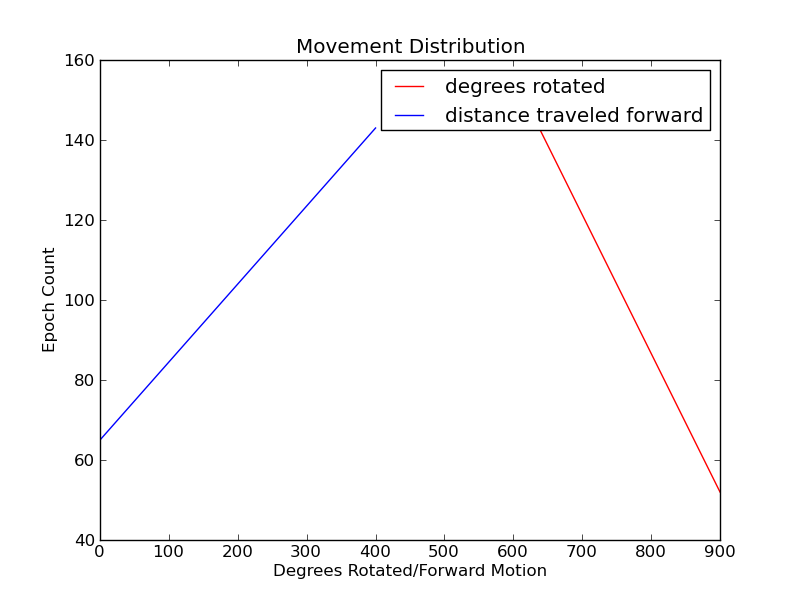
\includegraphics[scale=1.0]{img/brain3/travelGauss-r150.00-d200.00.png}
  \caption{Brain 3 Distribution of Number of Degrees Rotated and Units Travelled Forward per Epoch}
  \label{fig:b3travel}
\end{center}
\end{figure}

















%brain 4
\begin{figure}
\begin{center}
  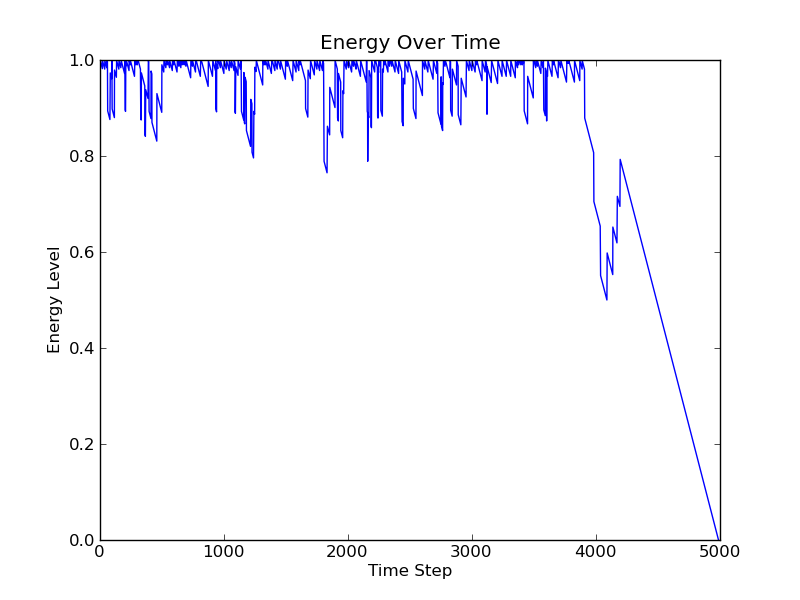
\includegraphics[scale=1.0]{img/brain4/1354432461-1.000000-EvT.png}
  \caption{Brain 4 Energy over Time for a Random Epoch}
  \label{fig:b4evt}
\end{center}
\end{figure}

\begin{figure}
\begin{center}
  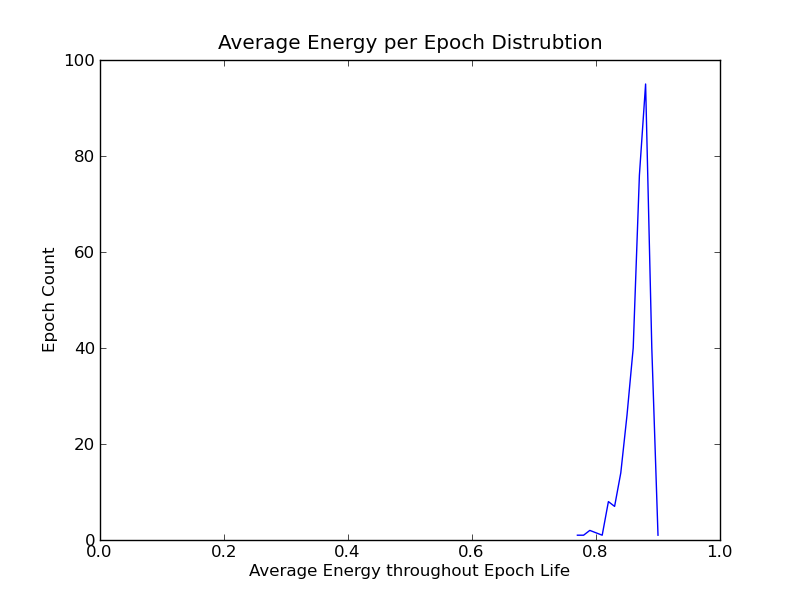
\includegraphics[scale=1.0]{img/brain4/avgenergyGauss-0.04.png}
  \caption{Brain 4 Distribution of Average Energies per Epoch}
  \label{fig:b4avgenergy}
\end{center}
\end{figure}

\begin{figure}
\begin{center}
  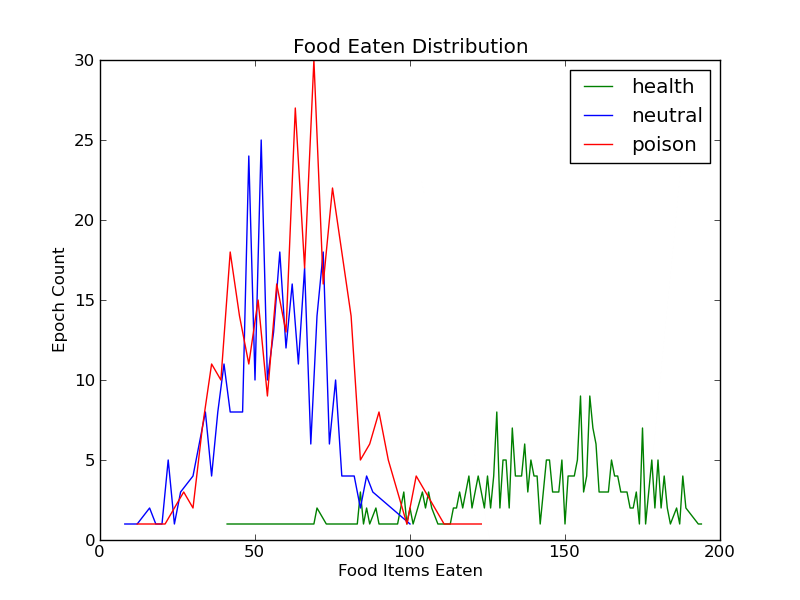
\includegraphics[scale=1.0]{img/brain4/foodGauss-h37.79-n23.82-p30.68.png}
  \caption{Brain 4 Distribution of Food Items Eaten per Epoch}
  \label{fig:b4food}
\end{center}
\end{figure}

\begin{figure}
\begin{center}
  \includegraphics[scale=1.0]{img/brain4/survivalGauss-3172.14.png}
  \caption{Brain 4 Distribution of Time Steps Survived per Epoch}
  \label{fig:b4survive}
\end{center}
\end{figure}

\begin{figure}
\begin{center}
  \includegraphics[scale=1.0]{img/brain4/travelGauss-r5389.65-d916.52.png}
  \caption{Brain 4 Distribution of Number of Degrees Rotated and Units Travelled Forward per Epoch}
  \label{fig:b4travel}
\end{center}
\end{figure}


















%brain 5
\begin{figure}
\begin{center}
  \includegraphics[scale=1.0]{img/brain5/1354471986-5.000000-EvT.png}
  \caption{Brain 5 Energy over Time for a Random Epoch}
  \label{fig:b5evt}
\end{center}
\end{figure}

\begin{figure}
\begin{center}
  \includegraphics[scale=1.0]{img/brain5/avgenergyGauss-0.07.png}
  \caption{Brain 5 Distribution of Average Energies per Epoch}
  \label{fig:b5avgenergy}
\end{center}
\end{figure}

\begin{figure}
\begin{center}
  \includegraphics[scale=1.0]{img/brain5/foodGauss-h27.29-n52.8-p31.64.png}
  \caption{Brain 5 Distribution of Food Items Eaten per Epoch}
  \label{fig:b5food}
\end{center}
\end{figure}

\begin{figure}
\begin{center}
  \includegraphics[scale=1.0]{img/brain5/survivalGauss-3872.22.png}
  \caption{Brain 5 Distribution of Time Steps Survived per Epoch}
  \label{fig:b5survive}
\end{center}
\end{figure}

\begin{figure}
\begin{center}
  \includegraphics[scale=1.0]{img/brain5/travelGauss-r7664.03-d1032.80.png}
  \caption{Brain 5 Distribution of Number of Degrees Rotated and Units Travelled Forward per Epoch}
  \label{fig:b5travel}
\end{center}
\end{figure}











%brain 6
\begin{figure}
\begin{center}
  \includegraphics[scale=1.0]{img/brain6/1355176281-0.250000-EvT.png}
  \caption{Brain 6 Energy over Time for a Random Epoch}
  \label{fig:b6evt}
\end{center}
\end{figure}

\begin{figure}
\begin{center}
  \includegraphics[scale=1.0]{img/brain6/avgenergyGauss-0.05.png}
  \caption{Brain 6 Distribution of Average Energies per Epoch}
  \label{fig:b6avgenergy}
\end{center}
\end{figure}

\begin{figure}
\begin{center}
  \includegraphics[scale=1.0]{img/brain6/foodGauss-h19.99-n5.74-p8.62.png}
  \caption{Brain 6 Distribution of Food Items Eaten per Epoch}
  \label{fig:b6food}
\end{center}
\end{figure}

\begin{figure}
\begin{center}
  \includegraphics[scale=1.0]{img/brain6/survivalGauss-3452.05.png}
  \caption{Brain 6 Distribution of Time Steps Survived per Epoch}
  \label{fig:b6survive}
\end{center}
\end{figure}

\begin{figure}
\begin{center}
  \includegraphics[scale=1.0]{img/brain6/travelGauss-r3203.12-d916.52.png}
  \caption{Brain 6 Distribution of Number of Degrees Rotated and Units Travelled Forward per Epoch}
  \label{fig:b6travel}
\end{center}
\end{figure}













%brain 7
\begin{figure}
\begin{center}
  \includegraphics[scale=1.0]{img/brain7/1354746755-0.250000-EvT.png}
  \caption{Brain 7 Energy over Time for a Random Epoch}
  \label{fig:b7evt}
\end{center}
\end{figure}

\begin{figure}
\begin{center}
  \includegraphics[scale=1.0]{img/brain7/avgenergyGauss-0.01.png}
  \caption{Brain 7 Distribution of Average Energies per Epoch}
  \label{fig:b7avgenergy}
\end{center}
\end{figure}

\begin{figure}
\begin{center}
  \includegraphics[scale=1.0]{img/brain7/foodGauss-h30.46-n6.32-p7.75.png}
  \caption{Brain 7 Distribution of Food Items Eaten per Epoch}
  \label{fig:b7food}
\end{center}
\end{figure}

\begin{figure}
\begin{center}
  \includegraphics[scale=1.0]{img/brain7/survivalGauss-6835.36.png}
  \caption{Brain 7 Distribution of Time Steps Survived per Epoch}
  \label{fig:b7survive}
\end{center}
\end{figure}

\begin{figure}
\begin{center}
  \includegraphics[scale=1.0]{img/brain7/travelGauss-r6482.71-d916.52.png}
  \caption{Brain 7 Distribution of Number of Degrees Rotated and Units Travelled Forward per Epoch}
  \label{fig:b7travel}
\end{center}
\end{figure}

\end{document}
















%\section{Appendix the second}



\end{sloppypar}

\begin{thebibliography}{9}

\bibitem{Anders}
  Anders, Torsten, and Eduardo R. Miranda. ``Constraint Programming Systems for Modeling Music Theories and Composition.'' \underline{ACM Computing Surveys} 43.4 (2011): 1:38.

\end{thebibliography}

\end{document}


